\section*{L1 Concept}

\begin{frame}{L1 Trigger Prerequisites}{}
	\begin{block}{Reduction from $1 MHz$ to $100 kHz$}
		\begin{itemize}
	  		\item Data quality checks
	  		\item Basic reconstruction
	  		\item Multi-detector algorithms possible
		\end{itemize}
	\end{block}
	
	\begin{exampleblock}{Time per event about $400\mu s - 1 ms$}
		\begin{itemize}
	  		\item 30 PCs * 16 cores
	  		\item About 2 cores used for the framework
	  		\item Burst time shared by L1/L2 
		\end{itemize}
	\end{exampleblock}
\end{frame}


\begin{frame}[fragile]
\frametitle{User interface: Decoder}
The framework provides a decoder for all detectors (so far only Tel-board based
data)

\begin{lstlisting}[frame=trBL,caption={}]{}
for (auto trb : decoderHandler.getCEDARDecoderRange()) {
    for(uint hit = 0; hit != trb->getNumberOfEdgesStored(); i++) {
        trb->getTimes()[hit];
        trb->getChIDs()[hit];
        trb->getTdcIDs()[hit];
        trb->getIsLeadings()[hit];
    }
}
\end{lstlisting}	
\end{frame}

\begin{frame}{Lazy Decoding}{}
	\begin{block}{Decoder methods are idempotent}
		\begin{itemize}
	  		\item Actual decoding processed only when user accesses data
	  		\item Data may be accessed in any order
	  		\item Decoding takes place only once
		\end{itemize}
	\end{block}
	\vspace{0.5cm}
	More info: \\
	github.com/NA62/na62-trigger-algorithms/wiki/Lazy-decoding
\end{frame}

\begin{frame}{Current performance}{}
	\begin{block}{Rough performance test (preliminary!)}
		\begin{itemize}
	  		\item Decoded CEDAR data with average of 6 edges per event
	  		\item Average decoding time: ~	$\sim 14 \mu s$ per Event
	  		\item Sums of all edges in every sector: $\sim 2 \mu s$ per Event
	  		\item Time dominated by cache misses
		\end{itemize}
	\end{block}
	Test was only singlethreaded (no load on PC)!
\end{frame}

%%%%%%%%%%%%%%%%%%%%%%%%%%%%%%%%%%%%%%%%%%%%%%%%%%%%%%%%%%%%%%%%%%%%%%%%%%%%%%%%%
\section*{Downscaling and Bypassing}

\begin{frame}{Bypassing}{}
	\begin{block}{Events may bypass L1/L2 with a configurable probability}
		\begin{itemize}
		  	\item Bypassing means accepting without processing
		  	\item Special L1/L2 trigger word stored for bypassed events
	  		\item Example: --L1BypassProbability=0.1
	  		\begin{itemize}
	  			\item 10\% of all events would be accepted without processing L1/L2
	  		\end{itemize} 
		\end{itemize}
	\end{block}
	\vspace{0.5cm}
	See github.com/NA62/na62-trigger-algorithms/wiki/TriggerBypassing
\end{frame}

\begin{frame}{Downscaling}{}
	Downscaling means rejecting without processing
	\begin{block}{Global L1/L2 downscaling}
		\begin{itemize}
		  \item E.g. --L1DownscaleFactor=3
		  \item Only every third event will be processed
		  \item Please try to use downscaling on the L0TP side instead!
		\end{itemize}
	\end{block}
	
	\begin{block}{Algorithm specific downscaling}
		\begin{itemize}
		  \item Every (detector specific) algorithm can be downscaled
		  \item E.g. --algodownscaling\_CEDAR=10
		\end{itemize}
	\end{block}
	
	\vspace{0.5cm}
	See github.com/NA62/na62-trigger-algorithms/wiki/Downscaling
\end{frame}


%%%%%%%%%%%%%%%%%%%%%%%%%%%%%%%%%%%%%%%%%%%%%%%%%%%%%%%%%%%%%%%%%%%%%%%%%%%%%%%%%
\section*{Data Formats}

\begin{frame}{New Burst File Format}{}
	\begin{block}{Added header on top of old format}
		\begin{itemize}
		  \item Format version (distinguishable from old format)
		  \item Number of Events stored
		  \item Rund and Burst ID
		  \item Three lookup tables
		  	\begin{itemize}
			  \item Eventnumbers
			  \item Trigger type word
			  \item Offset (pointer) 
			\end{itemize}
		\end{itemize}
	\end{block}
	This allows you to more quickly filter/access specific events	
\end{frame}

\begin{frame}{Burst File Header}{}
		\begin{figure}[htbp]
		  \centering
		  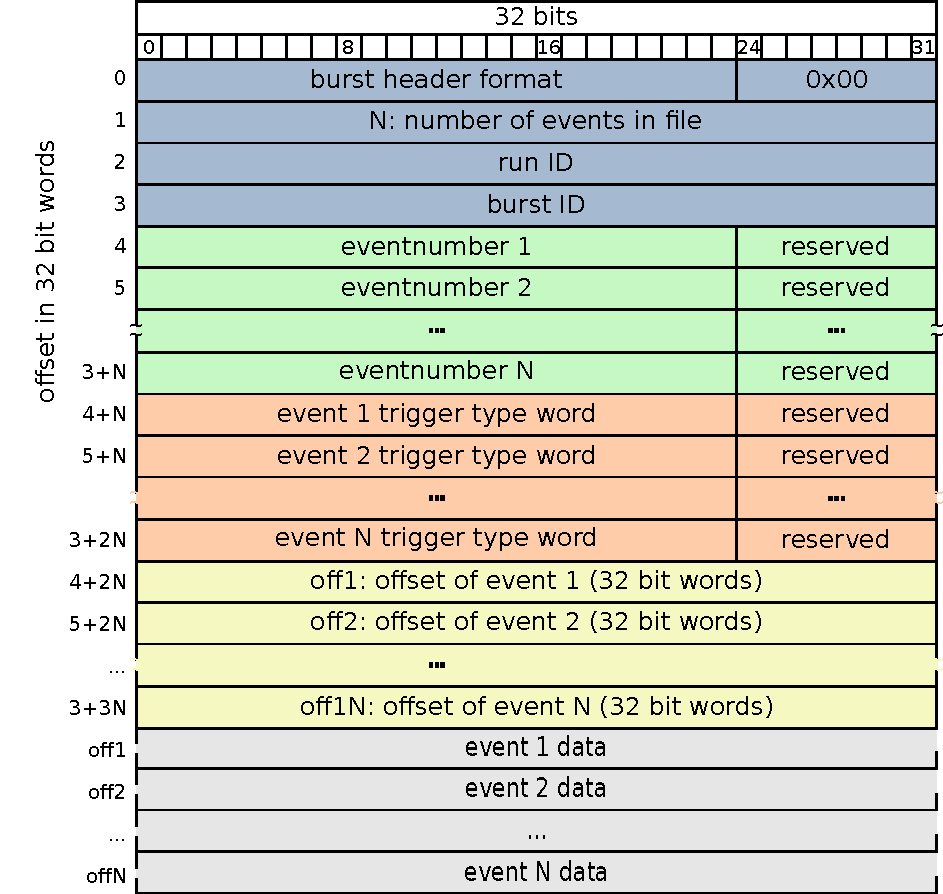
\includegraphics[width=0.8\textwidth]{BurstFileHeader.pdf}
		\end{figure}
\end{frame}


%%%%%%%%%%%%%%%%%%%%%%%%%%%%%%%%%%%%%%%%%%%%%%%%%%%%%%%%%%%%%%%%%%%%%%%%%%%%%%%%%
\section*{Activities/People}

\begin{frame}{People}{}
	\begin{block}{Implementation (for Tel62 readout sub-detectors):}
		\begin{itemize}
		  \item Main common framework + decoding handler: Jonas (done)
		  \item Tel62 Decoder: Angela (done)
		  \item Cedar: Angela (first version committed, investigating high intensity)
		  \item RICH: Valeria (ongoing)
		  \item MUV3: Valeria-Angela (ongoing)
		  \item CHOD? SAC? LAV?
		\end{itemize}
	\end{block}
\end{frame}

\begin{frame}{People}{}
	\begin{block}{Concept study (can use L0 output provided by Bruno)}
		\begin{itemize}
		  \item Cedar: Angela (ongoing)
		  \item RICH: Valeria (ongoing)
		  \item 1-Track (with combined info from CHOD-MUV): Tommaso (ongoing)
		\end{itemize}
	\end{block}
\end{frame}

\begin{frame}{Past Activities}{}
	\begin{block}{Tests already performed}
		\begin{itemize}
		  \item Crosscheck between offline and online reconstruction performed for
		  Cedar and RICH
		  \item Test of Cedar L1 trigger on PCfarm @ CERN - same DAQ and handling as during NA62
data taking
		  \item Test of simple algorithm involving two sub-detectors on PC farm (used Cedar and CHOD)
		\end{itemize}
	\end{block}
\end{frame}

\begin{frame}{Ongoing/Future Activities}{}
	\begin{block}{Ongoing Activities}
		\begin{itemize}
		  \item Test of L1 trigger on data (from 2014) and MC (from L0 output): understand comparison,
			accidentals and handling of corrupted data
			\item RICH L1 trigger concept study: is the MultiRing existing algorithm good
			enough?
			\item 1-Track L1 trigger concept study: is there a simple and fast algorithm to
			do that?
		\end{itemize}
	\end{block}
	
	\begin{block}{Future Activities}
		\begin{itemize}
			\item Implementation and Test of RICH L1 trigger (April/May)
			\item Test of L1 trigger @ CERN (April/May)
		\end{itemize}
	\end{block}
\end{frame}

%%%%%%%%%%%%%%%%%%%%%%%%%%%%%%%%%%%%%%%%%%%%%%%%%%%%%%%%%%%%%%%%%%%%%%%%%%%%%%%%%
\begin{frame}{So Long, and Thanks for All the Fish}{}
	\begin{block}{That was my last talk at CERN}
		Goodbye!
	\end{block}
\end{frame}